\section{Problem Definition, Data, and Evaluation Framework}\label{sec:v2-data}

\subsection{Problem Definition}\label{sec:v2-common-problem}

This work aims to build an intelligent system that predicts drug solubility under multiple conditions. Let the $i$-th physical measurement be the triple
\begin{equation}
x_i = (d_i, s_i, T_i),
\end{equation}
where $d_i \in \mathcal{D}$ is the canonical SMILES string of the drug, $s_i \in \mathcal{S}$ the canonical structure of the solvent, and $T_i \in \mathbb{R}$ the operating temperature in degrees Celsius. The measured response is the decimal molar log-solubility $y_i = \log_{10} S_i \in \mathbb{R}$ (the raw concentration is in $\mathrm{mol/L}$).

Two derived variables support the modelling and evaluation. The combination key $c_i = (d_i, s_i)$ identifies a specific drug--solvent system, inside which the molecular structures are fixed while the temperature and the measured solubility can vary continuously; the parent label $g_i \in \mathcal{G}$ isolates the scaffold in data splitting, sample weighting, and metric computation. The goal is to learn a mapping $f: \mathcal{D} \times \mathcal{S} \times \mathbb{R} \to \mathbb{R}$ that minimises the expected generalisation error on a novel parent $g^* \notin \mathcal{G}_{\mathrm{train}}$.

\subsection{Data and Quality Characteristics}

We use the course-provided benchmark \texttt{data\_2026.csv}, which holds 1904 real experimental measurements. Table~\ref{tab:v2-data-fields} summarises the raw fields and their roles in the pipeline.

\begin{table}[htbp]
  \centering\small
  \caption{Field definitions of the experimental dataset and their roles in the modelling pipeline.}
  \label{tab:v2-data-fields}
  \begin{tabularx}{\linewidth}{@{}lllX@{}}
    \toprule
    Field & Type & Unit / format & Role and handling \\
    \midrule
    \texttt{Drug} & string & pharmacopoeia / trade name & identity index and interface display. \\
    \texttt{Solvent} & string & common English name & solvent lookup and interface search. \\
    \texttt{Drug SMILES} & string & canonical structure & drug representation, descriptors, and parent parsing. \\
    \texttt{Solvent SMILES} & string & canonical structure & solvent representation and explicit physicochemical features. \\
    \texttt{Temperature} & float & $^\circ\text{C}$ & thermodynamic environment for continuous regression and condition scans. \\
    \texttt{Solubility\_log10} & float & $\log_{10}(\mathrm{mol/L})$ & regression target for training, tuning, and evaluation. \\
    \texttt{Solubility Unit} & category & $\mathrm{mol/L}$ & concentration-unit label used in the inverse transform. \\
    \bottomrule
  \end{tabularx}
\end{table}

A thorough audit confirms that all 1904 records parse successfully with RDKit and that neither the inputs nor the targets contain missing values. Physicochemically, the data exhibit three salient features:
the log-solubility $y$ spans $[-6.2343, 2.2168]$, a dynamic range of more than eight orders of magnitude, which demands numerical stability across a wide scale;
the data contain non-negligible conflicting repeated measurements: when canonical combinations and temperatures are matched exactly, 86 groups totalling 205 records carry different labels under the same nominal conditions, and 11 of those groups differ by more than one order of magnitude. These conflicts plausibly stem from differences across measurement batches in equilibration time, polymorphic state, or solid--liquid separation; the model keeps these records to test its tolerance to realistic noise;
the temperature window is broad, from $-59.5^\circ\text{C}$ to $130.0^\circ\text{C}$, with a median of $25.0^\circ\text{C}$ and an interquartile range of $20.0^\circ\text{C}$, giving ample temperature variation for uncovering the underlying physics.

\subsection{Parent Scaffold Standardisation}

In medicinal chemistry, one pharmacophore can appear in different salt forms, charge states, and stereoisomers. The raw data record 186 distinct drug names, which resolve to 168 unique molecular structures after SMILES canonicalisation.

To sever the hidden leakage among related scaffolds, we parse the parents deeply with RDKit's \texttt{ChargeParent} algorithm. The standardisation strips inactive solvates and inorganic counterions (such as $\mathrm{Cl}^-$, $\mathrm{Na}^+$), neutralises formal charges to the neutral parent, and removes cis/trans and chiral markers, leaving the pure topological parent. The full dataset then reduces strictly to 161 distinct parents, so that all salts and stereoisomers of one drug map to the same group key $g_i$ and the grouped cross-validation is physically airtight.

\subsection{Data Distribution and Sparsity}

Figure~\ref{fig:v2-data-overview} shows how the dataset covers chemical and condition space.

\begin{figure}[htbp]
  \centering
  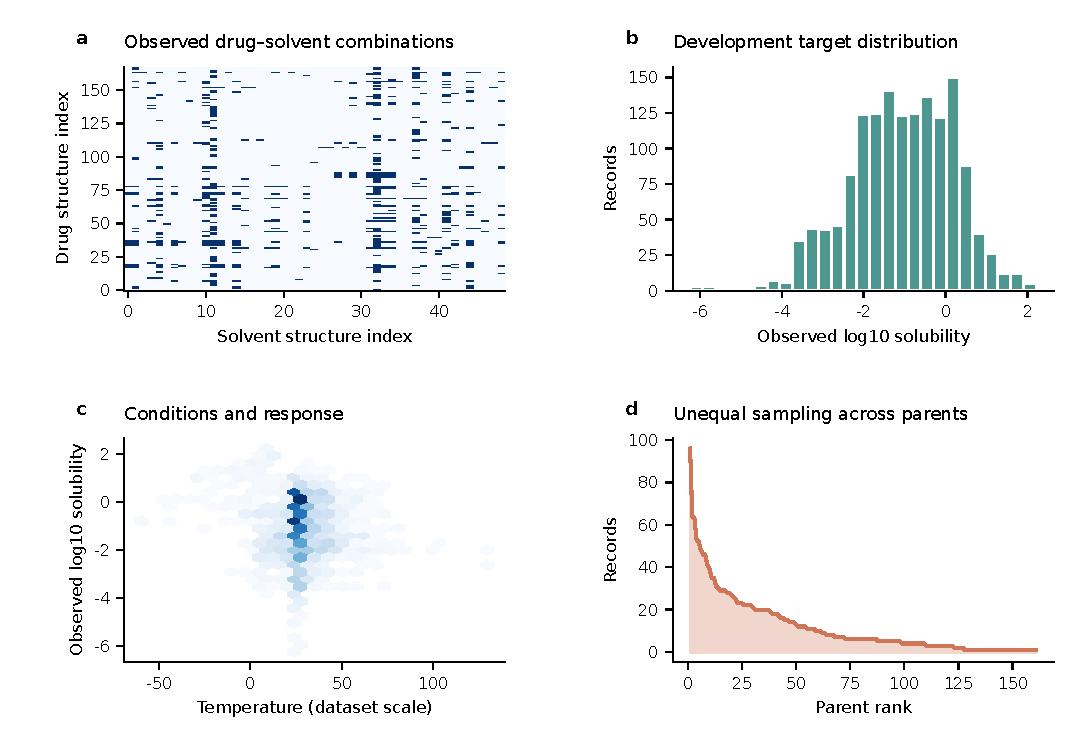
\includegraphics[width=\linewidth]{revision_v2/v2_data.pdf}
  \caption{Coverage, condition distribution, and sampling frequency of the dataset. \textbf{a} observed coverage of the drug--solvent combination grid; \textbf{b} log-solubility distribution of the development set; \textbf{c} joint temperature--solubility density; \textbf{d} descending per-parent sample counts.}
  \label{fig:v2-data-overview}
\end{figure}

Of the $168 \times 49 = 8232$ theoretical drug--solvent combinations, only 646 are actually observed, a global sparsity of 92.15\% (Figure~\ref{fig:v2-data-overview}a). Among these 646 combinations, 222 contain repeated measurements at several temperatures and account for 77.73\% of the rows, forming the core base for temperature-dependence analysis. The per-parent sample counts follow a sharp long-tail distribution (Figure~\ref{fig:v2-data-overview}d): 74 rare parents hold only 1--5 records each (182 records in total), while the top 30 parents each exceed 20 observations and monopolise 1078 records, 56.6\% of the dataset. Without reweighting and parent-equal evaluation, any conventional learner would inevitably overfit the head parents.

\subsection{Experimental Setup and Parent-Weighted Evaluation}\label{sec:v2-experiments}

\subsubsection{Nested Parent Holdout Design}
To balance strict anti-leakage against data use, the 161 parents are split in two: a core development set of 128 parents (1507 records) for model building, nested cross-validation, hyperparameter tuning, feature ablation, and blend-weight learning; and a held-out historical benchmark of 33 fully independent parents (397 records) as an unseen test library.

Within the development set, we adopt a strict five-outer/three-inner nested grouped cross-validation (Nested GroupKFold by parent). The outer loop splits parents into five folds, holding one out for unbiased evaluation; inside each outer training set, parents are again split into three inner folds, and all standardisation, imputation, dimensionality reduction, hyperparameter search, and blend-weight selection happen inside the inner loop\cite{varma2006,cawley2010}, keeping the outer validation fold invisible throughout. The outer models are refit under three random seeds (2026, 17, 42) to gauge the variance from algorithmic randomness.

\subsubsection{Parent-Weighted Risk and Sample Reweighting}
To counter long-tailed sampling, we formalise a parent-weighted empirical risk. Let $\mathcal{G}$ be the validation parents and $I_g$ the indices of all samples belonging to parent $g \in \mathcal{G}$. The evaluation loss is
\begin{equation}\label{eq:v2-common-risk}
\mathcal{L}_{\mathcal{G}}(f) = \frac{1}{|\mathcal{G}|} \sum_{g \in \mathcal{G}} \left( \frac{1}{|I_g|} \sum_{i \in I_g} |y_i - f(x_i)| \right).
\end{equation}
This criterion averages the absolute error inside each parent and then gives every parent exactly equal weight ($1/|\mathcal{G}|$), so that the metric reflects average generalisation over novel parents rather than being swayed by the parents with the most records.

To align the tree-splitting objective with this criterion, training uses the adaptive sample weight
\begin{equation}
w_i(q) = \frac{n_{g_i, \mathcal{T}}^{-q}}{N_{\mathcal{T}}^{-1} \sum_{j \in \mathcal{T}} n_{g_j, \mathcal{T}}^{-q}}, \qquad q \in \{0, 1\},
\label{eq:v2-train-weight}
\end{equation}
where $\mathcal{T}$ is the current training fold, $n_{g, \mathcal{T}}$ the number of samples of parent $g$ in $\mathcal{T}$, and $N_{\mathcal{T}} = |\mathcal{T}|$. With $q=0$ this reduces to ordinary row weighting; with $q=1$ each parent contributes a constant $N_{\mathcal{T}}/G_{\mathcal{T}}$ to the total loss regardless of how many records it has.

\subsubsection{Evaluation Metrics and Paired Inference}
Four metrics summarise the results. The parent-weighted mean absolute error (where $A_g = \frac{1}{|I_g|}\sum_{i\in I_g}|e_i|$ is parent $g$'s mean absolute error):
\begin{equation}
\mathrm{MAE}_{\mathrm{parent}} = \frac{1}{G}\sum_{g=1}^G A_g,
\end{equation}
the row-wise mean absolute error:
\begin{equation}
\mathrm{MAE}_{\mathrm{row}} = \frac{1}{N}\sum_{i=1}^N |e_i|,
\end{equation}
the root-mean-square error:
\begin{equation}
\mathrm{RMSE} = \sqrt{\frac{1}{N}\sum_{i=1}^N e_i^2},
\end{equation}
and the coefficient of determination:
\begin{equation}
R^2 = 1 - \frac{\sum_{i=1}^N e_i^2}{\sum_{i=1}^N (y_i - \bar y)^2}.
\end{equation}

Model comparisons use a non-parametric parent-paired bootstrap. Over 10,000 resamples of the 128 outer parents, we compute the paired difference $\Delta = \frac{1}{G}\sum_{g=1}^G (A_{g, A} - A_{g, B})$ and take the 2.5\% and 97.5\% quantiles as a 95\% confidence interval, which certifies the statistical significance of any improvement.

\subsection{Overall Architecture}

On a shared data structure and evaluation basis, this work builds and contrasts two complementary routes: SOLAR-H extracts the physical temperature slope by within-combination de-meaning, while ExtraTrees--TabPFN pursues high-dimensional explicit feature engineering and tabular-model blending (overview in Figure~\ref{fig:v2-method-workflows}).

\begin{figure}[htbp]
\centering
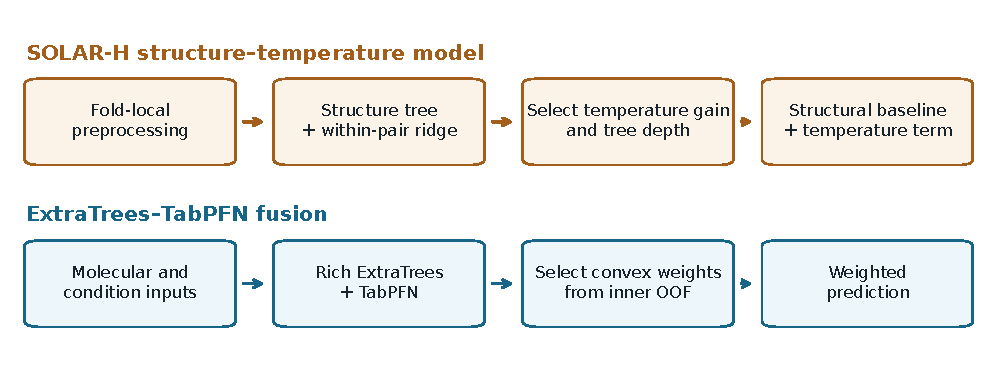
\includegraphics[width=\linewidth]{method_workflows.pdf}
\caption{Overview of the two technical routes for conditional solubility prediction.}
\label{fig:v2-method-workflows}
\end{figure}
